\documentclass[12pt]{article}

\usepackage{fullpage}
\usepackage{fancybox}
\usepackage{amssymb}
\usepackage{amsmath}
\usepackage{graphicx}

\newcommand{\BS}{\textsf{\sc BieberSearch}}

\newcommand{\IE}{\mathbb{E}}

%%%%%%%%%%%%Separating rule above/below figures%%%%%%%%%%%%%%%%%%%%%
\setlength{\textfloatsep}{5ex}
\newcommand{\topfigrule}{\noindent\rule[-0.5cm]{\textwidth}{0.2mm}\vspace*{-6pt}\noindent}
\newcommand{\botfigrule}{\noindent\rule[-0.5cm]{\textwidth}{0.2mm}}
%%%%%%%%%%%%%%%%%%%%%%%%%%%%%%%%%%%%%%%%%%%%%%%%%%%%%%%%%%%%%%%%%%%%

%%%%%%%%%%%%%% Capsule %%%%%%%%%%%%%%%%%%%%%%%%%%%%%%%%%%%%%%%%%%%
\newcommand{\capsule}[2]{\vspace{0.5em}
  \shadowbox{%
    \begin{minipage}{.90\linewidth}%
      \textbf{#1:}~#2%
    \end{minipage}}
  \vspace{0.5em} }
%%%%%%%%%%%%%%%%%%%%%%%%%%%%%%%%%%%%%%%%%%%%%%%%%%%%%%%%%%%%%%%%%%

\newcounter{ques}
\newenvironment{question}{\stepcounter{ques}{\noindent\bf Question \arabic{ques}:}}{\vspace{5mm}}
\newenvironment{solution}{{\noindent\bf Solution:}}{\vspace{5mm}}


\begin{document} 

\begin{center} \Large\bf
COMP 3804 --- Assignment 1 
\end{center} 

\noindent {\bf Due:} Thursday February 2, 23:59.

\vspace{0.5em}

\noindent {\bf Assignment Policy:}
\begin{itemize}
\item Your assignment must be submitted as one single PDF file through
      Brightspace.

\begin{center}
\shadowbox{
  \begin{minipage}{.90\linewidth}
    {\textsf{Use the following format to name your file: 
        \[ {\tt LastName\_StudentId\_a1.pdf}
        \] 
      }}
  \end{minipage}
}
\end{center}
\item {\bf Late assignments will not be accepted. I will not reply to
      emails of the type ``my internet connection broke down at
      23:57'' or ``my scanner stopped working at 23:58'', or
      ``my dog ate my laptop charger''.}
\item You are encouraged to collaborate on assignments, but at the level
      of discussion only. When writing your solutions, you must do so
      in your own words.
\item Past experience has shown conclusively that those who do not put
      adequate effort into the assignments do not learn the material and
      have a probability near 1 of doing poorly on the exams.
\item When writing your solutions, you must follow the guidelines below.
      \begin{itemize}
      \item You must justify your answers.
      \item The answers should be concise, clear and neat.
      \item When presenting proofs, every step should be justified.
      \end{itemize}
\end{itemize}

\begin{center}
\shadowbox{
  \begin{minipage}{.90\linewidth}
    {\textsf{Some useful facts:
      \begin{enumerate}
         \item for any real number $x>0$, $x = 2^{\log x}$. 
         \item For any real number $x \neq 1$ and any integer $k \geq 1$, 
               \[ 1 + x + x^2 + \cdots + x^{k-1} = \frac{x^k - 1}{x-1} . 
               \]
         \item For any real number $0 < \alpha < 1$, 
               \[ \sum_{i=0}^{\infty} \alpha^i = \frac{1}{1-\alpha} . 
               \] 
      \end{enumerate}
      }}
  \end{minipage}
}
\end{center}

\newpage 

\begin{question}
Write your name and student number. \newline

\begin{solution}
      Ryan Lo (101117765)
\end{solution}

\end{question}

\begin{question} 
Consider the following recurrence, where $n$ is a power of $6$: 
\[ T(n) = \left\{ \begin{array}{ll} 
                    1 & \mbox{if $n=1$,} \\ 
                    n^2 + 11 \cdot T(n/6) & \mbox{if $n \geq 6$.} 
                  \end{array} 
          \right. 
\]

\begin{itemize} 
\item Solve this recurrence using the \emph{unfolding method}. 
Give the final answer using Big-O notation.  

$T(n) = n^2 + 11 * T(n/6)$

$T(n) = n^2 + 11 (({n/6})^2 + 11 *T(n/6^2))$

$T(n) = n^2 + 11({n/6})^2 + 11^2 * T(n/6^2)$

$T(n) = (1 + 11/6^2) n^2 + 11^2 * T(n/6^2)$

$T(n) = (1 + 11/6^2) n^2 + 11^2 * ((n/6^2)^2 + 11 * T(n/6^3))$

$T(n) = (1 + 11/6^2 + 11^2/6^4) n^2 + 11^3 * T(n/6^3)$

$T(n) = (1 + 11/6^2 + 11^2/6^4) n^2 + 11^3 * ((n/6^3)^2 + 11 * T(n/6^4))$

$T(n) = (1 + 11/6^2 + 11^2/6^4 + 11^3/6^6) n^2 + 11^4 * T(n/6^4)$

.
.
.

$T(n) = (1 + 11/6^2 + 11^2/6^4 + ... + 11^{k-1}/6^{2(k-1)}) n^2 + 11^k * T(n/6^{k})$

$T(n/6^{k}) = T(1)$

$T(n) \leq \sum_{i=0}^{k-1}11^i/6^{2i} n^2 + 6^k * T(1)$

$= \frac{(11/6^2)^k - 1}{(11/6^2) - 1}1/1-(11/6^2) n^2 + 6^k$

$= \frac{36}{25} n^2 + n$

$= O(n^2)$

\item Solve this recurrence using the \emph{Master Theorem}. 
\end{itemize} 

$a = 11, b = 6, d = 2$

if $d > log_b a : T(n) = O(n^d)$

$2 > log_6 11$

$2 > 1.3383$

$T(n) = O(n^2)$

\end{question} 

\begin{question} 
Consider the following recurrence:  
\[ T(n) = n + T(n/5) + T(7n/10) . 
\]
In class, we have seen that $T(n) = O(n)$. In this question, you will 
prove this using the \emph{recursion tree method}. 

Recall from class: The root represents the recursion tree on an input 
of size $n$. Consider a node $u$ in the recursion tree that represents 
a recursive call on an input of size $m$. Then we write the value $m$ 
at this node $u$, we give $u$ a left subtree which is a recursion tree 
for an input of size $m/5$, and we give $u$ a right subtree which is a 
recursion tree for an input of size $7m/10$. In this way, $T(n)$ is the 
sum of the values stored at all nodes in the entire recursion tree. 

Below, we assume that the \emph{levels} in the recursion tree are 
numbered $0,1,2,\ldots,$, where the root is at level $0$. For each 
$i \geq 0$, let $S_i$ be the sum of the values of all nodes at level 
$i$. 
 
\begin{itemize}
\item Determine $S_0$. 
\item Determine $S_1$. 
\item Determine $S_2$. 
\item Use induction to prove the following claim: For every $i \geq 0$, 
\[ S_i \leq (9/10)^i \cdot n . 
\] 

\noindent \emph{Hint:} Consider level $i$, let $k = 2^i$, and let the 
values stored at the nodes at level $i$ be $m_1,m_2,\ldots,m_k$. 
What are the values stored at the nodes at level $i+1$? 
\item Complete the proof by showing that $T(n) = O(n)$. 
\end{itemize} 



$O(n)$

\end{question} 

\begin{solution}

      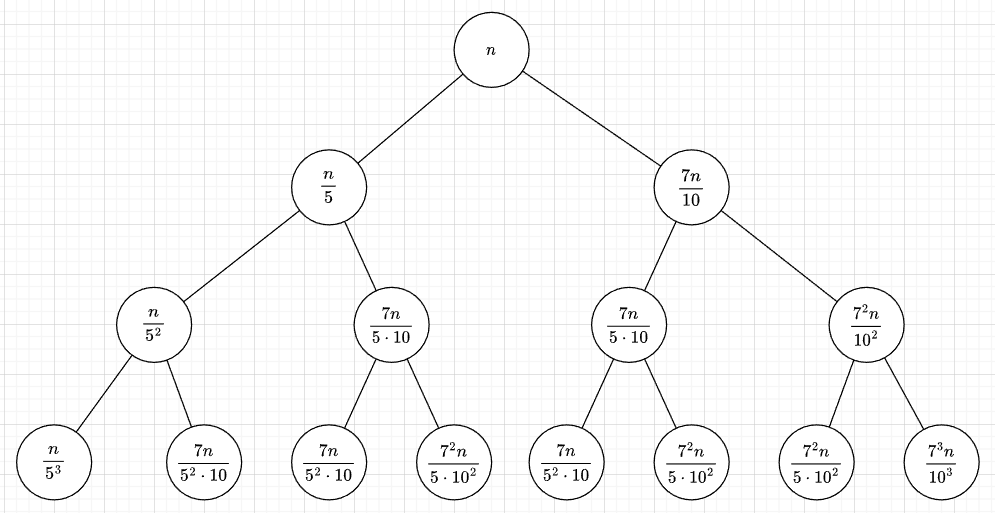
\includegraphics[width=150mm]{a1tree.png}

      The values stored at the nodes at level i + 1 are:

      $(1/5^i)n$, $(7/5^{i-1}*10)n$, $(7^{i-1}/5*10^{i-1})n$, $(7^i/5*10^i)n$

      $S_0 = n$

      $S_1 = (9/10)n$

      $S_2 = (9/10)^2 n$

      $S_3 = (9/10)^3 n$

      $n/5^k = 1$

      $k = log_5 n$

      $n/(7/10)^k = 1$

      $k_2 = log_{10/7} n$

      $T(n)= n + (9/10)n + (9/10)^2 n + ... + (9/10)^k n$

      $= n[1 + (9/10) + (9/10)^2 + ... + (9/10)^k]$

      $T(n) = O(n)$

\end{solution}

\begin{question} 
Zoltan is not only your friendly TA, he is also the owner of the popular 
budget airline ZoltanJet that offers flights in Canada. As you all know, 
there are $n$ airports in Canada. We denote these airports, in order from 
west to east, by $A_1,A_2,\ldots,A_n$. 

William, who is the CEO of ZoltanJet, has designed a \emph{flight plan} 
which is a list of ordered pairs $(A_i,A_j)$ of airports such that there 
is a direct flight from $A_i$ to $A_j$. This flight plan has the 
following two properties: 
\begin{itemize}
\item (P.1) Every flight is going 
      eastwards\footnote{But how do I get home? A customer service 
      representative will tell you ``that is your problem''.}. 
      In other words, if $(A_i,A_j)$ is in the flight plan, then $i<j$. 
\item (P.2) For any two indices $i$ and $j$ with $1 \leq i < j \leq n$, 
      it is possible to fly from $A_i$ to $A_j$ in at most two 
      \emph{hops}. In other words, either $(A_i,A_j)$ is in the flight 
      plan, or there is an index $k$ such that both $(A_i,A_k)$ and 
      $(A_k,A_j)$ are in the flight plan. Note that, because of (P.1), 
      $i < k < j$. 
\end{itemize}
Observe that ZoltanJet can guarantee (P.1) and (P.2) by offering 
direct flights between all ${n \choose 2} = \Theta(n^2)$ pairs 
$(A_i,A_j)$ of airports, where $1 \leq i < j \leq n$. 

\begin{itemize}
\item  
\noindent
Prove that ZoltanJet can guarantee (P.1) and (P.2) using a flight plan 
having only $O(n \log n)$ pairs of airports. You may assume that $n$ is a 
power of two.  

\noindent \emph{Hint:} Since this is the divide-and-conquer assignment, 
you probably have to use $\ldots$
\end{itemize}

\begin{solution}
      
      From P.1 we can imagine it as a sorted array of airports. 
      Now we can take P.2 and since it is possible to fly between 
      $A_i$ to $A_j$ in at most two hops, we can randomly partition it into 3 parts.
      Where the flight starts in the first partition hops into the second partition,
      then hops towards the third partition. Dividing it into 3 parts gives us
      $log_3 n$ and the case of having to visit every airports $n$.
      
      We get n traversals over every airport and n/3 partitions everytime so $O(nlogn)$ 


\end{solution}

\end{question}

\begin{question}
Professor Justin Bieber needs a fast algorithm that searches for an 
arbitrary element $x$ in a sorted array $A[1 \ldots n]$ of $n$ numbers. 
He remembers that there is something called ``binary search'', 
which maintains an interval $[\ell,r]$ of indices such that, if 
$x$ is present in the array, then it is contained in the subarray 
$A[\ell \ldots r]$. In one iteration, the algorithm takes the 
middle index, say $p$, in the interval $[\ell,r]$. Then the 
algorithm either finds $x$ at the position $p$, or it recurses in 
the interval $[\ell,p-1]$, or it recurses in the interval 
$[p+1,r]$. Unfortunately, Professor Bieber does not remember the 
expression\footnote{is it 
$\lfloor (r - \ell)/2 \rfloor$, or 
$\lceil (r - \ell)/2 \rceil$, or 
$\lfloor (r - \ell +1)/2 \rfloor$, or 
$\lceil (r - \ell +1)/2 \rceil$? 
}
for $p$ in terms of $\ell$ and~$r$. 

Professor Bieber does remember that, instead of choosing $p$ in the 
middle of the interval $[\ell,r]$, it is often enough to choose $p$ 
uniformly at random in this interval. Based on this, he obtains the 
following algorithm: The input consists of the sorted array 
$A[1 \ldots n]$, its size $n$, and a number $x$. If $x$ is in the array, 
then the algorithm returns the index $p$ such that $A[p]=x$. Otherwise, 
the algorithm returns ``not present''. We assume that all numbers in 
$A$ are distinct. 

\newpage 

\begin{quote}
\begin{tabbing}
{\bf Algorithm} $\BS(A,n,x)$:  \\
$\ell = 1$; $r = n$; \\
{\bf while} $\ell \leq r$ \\
{\bf do} \= $p=$ uniformly random element in
            $\{\ell,\ell+1,\ldots,r\}$; \\
         \> {\bf if} $A[p]<x$ \\
         \> {\bf then} $\ell = p+1$ \\
         \> {\bf else} \= {\bf if} $A[p]>x$ \\
         \>            \> {\bf then} $r=p-1$ \\
         \>            \> {\bf else} return $p$ \\
         \>            \> {\bf endif} \\
         \> {\bf endif} \\
{\bf endwhile}; \\
return ``not present''
\end{tabbing}
\end{quote}

Let $T$ be the running time of this algorithm on an input array of 
length $n$. Note that $T$ is a random variable. Prove that the expected 
value of $T$ is $O(\log n)$.

\noindent \emph{Hint:} Most solutions that you find on the internet 
are wrong. 
\end{question}

\begin{solution}
      
      A is a sorted array of n numbers. x is the element that we are searching for.

      We are going to show: $E(T) = O(log n)$

      When we run $BieberSearch(A,n,x)$, recursive calls are generated on smaller and smaller arrays.

      The expected time value of T considers all the cases where we get x.

      After 1 run, 2 runs, 3 runs, ..., n runs.

      Using the linearity of expectation we get:

      $T(n) = T(1) + T(2) + T(3) + ... + T(n)$

      $T(n) = 1 + 1/2 + 1/3 + ... + 1/n-1$

      This is actually a case of the harmonic numbers. The sum of the reciprocals becomes log n.

      $T(n) = O(logn)$

\end{solution}


\begin{question}
You are given a sequence $S$ consisting of $n$ numbers; not all of these 
numbers need to be distinct. 

Describe an algorithm, in plain English, that decides, in $O(n)$ time, 
whether or not this sequence $S$ contains a number that occurs more 
than $n/4$ times. 

You may use any result that was proven in class. Justify the correctness
of your algorithm and explain why the running time is $O(n)$. 

\noindent \emph{Hint:} The algorithm must be comparison-based; you are
not allowed to use hashing, bucket-sort, or radix-sort. 
\end{question}

\begin{solution}
    We can start with finding the median using the selection algorithm that we learned in class.
    We first find the median(m) then create a 3-way partition based on that median. Where we have the first partition as
    $|<m|, |=m|, |>m|$.
    If the median(m) is the element that we are looking for then we are finished looking.
    Otherwise, we can call this algorithm on both sides of the partition $|<m|, |>m|$.
    Once we find the element we can count if the equal partition contains more than $n/4$ of that element.
    If we find the element as the median then it is finished otherwise the element does not exist where it occurs more than $n/4$ times
    because dividing it into another 3-way partition will not have enough elements for $n/4$.
    Finding out the median takes $O(n)$ time, running the algorithm again on the right and left sides takes $2 * O(n)$ time.
    In total it takes $3*O(n)$ which is just $O(n)$.
    
\end{solution}

\end{document} 